\documentclass{article}\usepackage[]{graphicx}\usepackage[]{color}
%% maxwidth is the original width if it is less than linewidth
%% otherwise use linewidth (to make sure the graphics do not exceed the margin)
\makeatletter
\def\maxwidth{ %
  \ifdim\Gin@nat@width>\linewidth
    \linewidth
  \else
    \Gin@nat@width
  \fi
}
\makeatother

\definecolor{fgcolor}{rgb}{0.345, 0.345, 0.345}
\newcommand{\hlnum}[1]{\textcolor[rgb]{0.686,0.059,0.569}{#1}}%
\newcommand{\hlstr}[1]{\textcolor[rgb]{0.192,0.494,0.8}{#1}}%
\newcommand{\hlcom}[1]{\textcolor[rgb]{0.678,0.584,0.686}{\textit{#1}}}%
\newcommand{\hlopt}[1]{\textcolor[rgb]{0,0,0}{#1}}%
\newcommand{\hlstd}[1]{\textcolor[rgb]{0.345,0.345,0.345}{#1}}%
\newcommand{\hlkwa}[1]{\textcolor[rgb]{0.161,0.373,0.58}{\textbf{#1}}}%
\newcommand{\hlkwb}[1]{\textcolor[rgb]{0.69,0.353,0.396}{#1}}%
\newcommand{\hlkwc}[1]{\textcolor[rgb]{0.333,0.667,0.333}{#1}}%
\newcommand{\hlkwd}[1]{\textcolor[rgb]{0.737,0.353,0.396}{\textbf{#1}}}%
\let\hlipl\hlkwb

\usepackage{framed}
\makeatletter
\newenvironment{kframe}{%
 \def\at@end@of@kframe{}%
 \ifinner\ifhmode%
  \def\at@end@of@kframe{\end{minipage}}%
  \begin{minipage}{\columnwidth}%
 \fi\fi%
 \def\FrameCommand##1{\hskip\@totalleftmargin \hskip-\fboxsep
 \colorbox{shadecolor}{##1}\hskip-\fboxsep
     % There is no \\@totalrightmargin, so:
     \hskip-\linewidth \hskip-\@totalleftmargin \hskip\columnwidth}%
 \MakeFramed {\advance\hsize-\width
   \@totalleftmargin\z@ \linewidth\hsize
   \@setminipage}}%
 {\par\unskip\endMakeFramed%
 \at@end@of@kframe}
\makeatother

\definecolor{shadecolor}{rgb}{.97, .97, .97}
\definecolor{messagecolor}{rgb}{0, 0, 0}
\definecolor{warningcolor}{rgb}{1, 0, 1}
\definecolor{errorcolor}{rgb}{1, 0, 0}
\newenvironment{knitrout}{}{} % an empty environment to be redefined in TeX

\usepackage{alltt}
\usepackage{Sweave}
\usepackage{float}
\usepackage{graphicx}
\usepackage{tabularx}
\usepackage{siunitx}
\usepackage{mdframed}
\usepackage{amsmath}
\usepackage{gensymb}
\usepackage{natbib}
\bibliographystyle{..//refs/styles/besjournals.bst}
\usepackage[small]{caption}
\setkeys{Gin}{width=0.8\textwidth}
\setlength{\captionmargin}{30pt}
\setlength{\abovecaptionskip}{0pt}
\setlength{\belowcaptionskip}{10pt}
\topmargin -1.5cm        
\oddsidemargin -0.04cm   
\evensidemargin -0.04cm
\textwidth 16.59cm
\textheight 21.94cm 
%\pagestyle{empty} %comment if want page numbers
\parskip 7.2pt
\renewcommand{\baselinestretch}{1.5}
\parindent 0pt

\newmdenv[
  topline=true,
  bottomline=true,
  skipabove=\topsep,
  skipbelow=\topsep
]{siderules}

%% R Script


\IfFileExists{upquote.sty}{\usepackage{upquote}}{}
\begin{document}

\renewcommand{\thetable}{\arabic{table}}
\renewcommand{\thefigure}{\arabic{figure}}
\renewcommand{\labelitemi}{$-$}
%%%%%%%%%%%%%%%%%%%%%%%%%%%%%%%%%%%%%%%%%%%%%%%%%%%%%%%%%%%%%%%%%%%%%%%%%%%%%%%%%%%%%%%%%%%
\section*{US-NPN Timeline Figures}

\begin{figure} [H]
\begin{center}
\caption{Day of budburst and the day of leaf out for native tree species in New England. Data was collected from a growth chamber experiment using any combination of two photoperiod treatments, two forcing treatments, and three chilling treatments. The standard deviation is represented in blue for budburst and green for leaf out. }
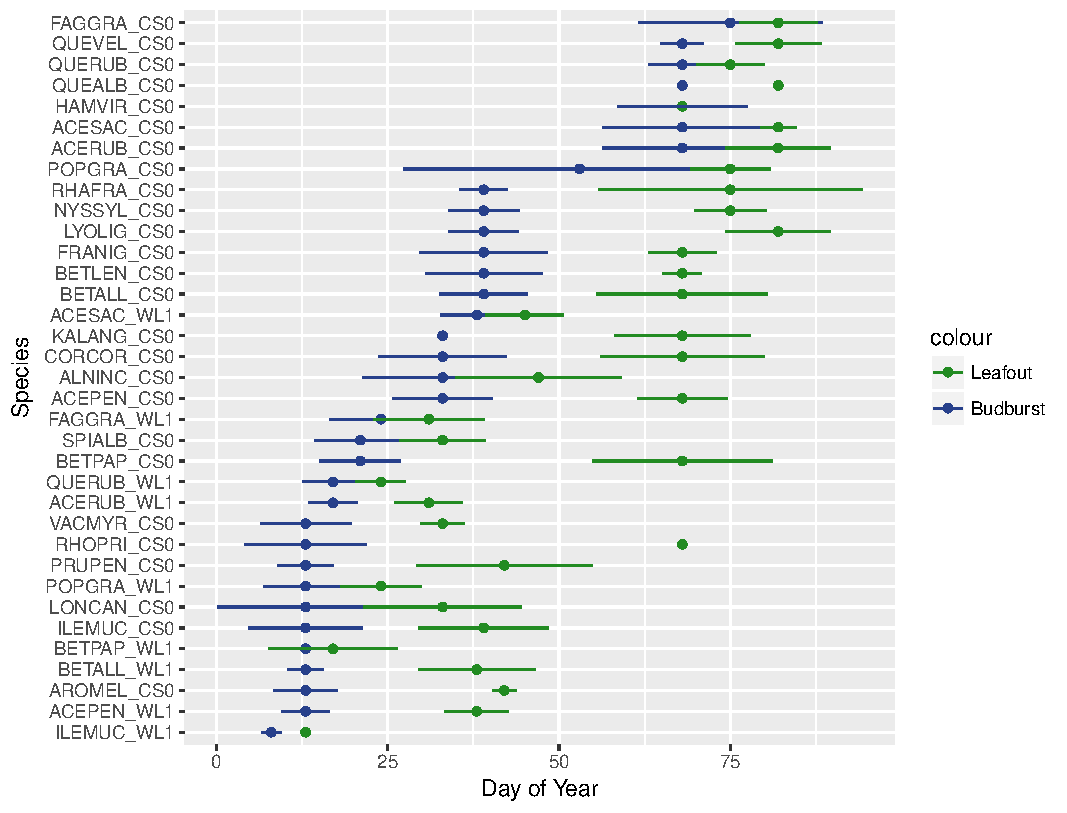
\includegraphics{..//output/Dan_TXandSp.pdf} 
\end{center}
\end{figure}


Anova Table (Type II tests)

Response: risk
          Sum Sq  Df F value    Pr(>F)    
chilling   119.1   1  1.9246    0.1682    
warm      4883.5   1 78.8970 1.602e-14 ***
photo     1300.3   1 21.0076 1.235e-05 ***
Residuals 6684.9 108                      
---
Signif. codes:  0 '***' 0.001 '**' 0.01 '*' 0.05 '.' 0.1 ' ' 1
Anova Table (Type II tests)

Response: risk
          Sum Sq  Df F value    Pr(>F)    
chilling     0.6   1  0.0094  0.923076    
warm      1742.3   1 26.3542 1.402e-06 ***
photo      462.9   1  7.0015  0.009461 ** 
Residuals 6611.2 100                      
---
Signif. codes:  0 '***' 0.001 '**' 0.01 '*' 0.05 '.' 0.1 ' ' 1
Anova Table (Type II tests)

Response: risk
          Sum Sq Df F value Pr(>F)  
chilling    15.5  1  0.2174 0.6426  
warm       269.9  1  3.7758 0.0564 .
photo      224.8  1  3.1453 0.0809 .
Residuals 4574.7 64                 
---
Signif. codes:  0 '***' 0.001 '**' 0.01 '*' 0.05 '.' 0.1 ' ' 1
Anova Table (Type II tests)

Response: risk
          Sum Sq Df F value  Pr(>F)  
chilling          0                  
warm      1025.1  1  5.9585 0.01929 *
photo      198.5  1  1.1541 0.28930  
Residuals 6709.5 39                  
---
Signif. codes:  0 '***' 0.001 '**' 0.01 '*' 0.05 '.' 0.1 ' ' 1
Anova Table (Type II tests)

Response: risk
          Sum Sq Df F value    Pr(>F)    
chilling          0                      
warm      374.08  1  40.041 0.0001364 ***
photo     126.75  1  13.567 0.0050493 ** 
Residuals  84.08  9                      
---
Signif. codes:  0 '***' 0.001 '**' 0.01 '*' 0.05 '.' 0.1 ' ' 1
Anova Table (Type II tests)

Response: risk
          Sum Sq  Df F value    Pr(>F)    
chilling   287.1   1  5.3166 0.0226709 *  
warm      1464.4   1 27.1142 7.109e-07 ***
photo      617.1   1 11.4266 0.0009506 ***
Residuals 7183.3 133                      
---
Signif. codes:  0 '***' 0.001 '**' 0.01 '*' 0.05 '.' 0.1 ' ' 1
Anova Table (Type II tests)

Response: risk
           Sum Sq Df F value    Pr(>F)    
chilling           0                      
warm      1383.03  1 18.8814 0.0003139 ***
photo      539.58  1  7.3665 0.0133581 *  
Residuals 1464.97 20                      
---
Signif. codes:  0 '***' 0.001 '**' 0.01 '*' 0.05 '.' 0.1 ' ' 1
Anova Table (Type II tests)

Response: risk
           Sum Sq  Df F value    Pr(>F)    
chilling      4.6   1  0.0554 0.8142417    
warm       1780.6   1 21.6850 7.928e-06 ***
photo      1104.1   1 13.4457 0.0003587 ***
Residuals 10510.5 128                      
---
Signif. codes:  0 '***' 0.001 '**' 0.01 '*' 0.05 '.' 0.1 ' ' 1
Anova Table (Type II tests)

Response: risk
           Sum Sq Df F value    Pr(>F)    
chilling           0                      
warm       941.67  1  14.261 0.0005059 ***
photo      660.25  1   9.999 0.0029452 ** 
Residuals 2707.30 41                      
---
Signif. codes:  0 '***' 0.001 '**' 0.01 '*' 0.05 '.' 0.1 ' ' 1
Anova Table (Type II tests)

Response: risk
           Sum Sq Df F value    Pr(>F)    
chilling    60.29  1  1.3655 0.2467952    
warm       722.34  1 16.3610 0.0001396 ***
photo        2.08  1  0.0472 0.8287207    
Residuals 2913.91 66                      
---
Signif. codes:  0 '***' 0.001 '**' 0.01 '*' 0.05 '.' 0.1 ' ' 1
Anova Table (Type II tests)

Response: risk
           Sum Sq Df F value    Pr(>F)    
chilling           0                      
warm      1094.34  1  23.115 2.416e-05 ***
photo      519.11  1  10.965  0.002043 ** 
Residuals 1799.04 38                      
---
Signif. codes:  0 '***' 0.001 '**' 0.01 '*' 0.05 '.' 0.1 ' ' 1
Anova Table (Type II tests)

Response: risk
          Sum Sq Df F value  Pr(>F)  
chilling          0                  
warm       92.04  1  3.3681 0.08067 .
photo       5.04  1  0.1845 0.67192  
Residuals 573.88 21                  
---
Signif. codes:  0 '***' 0.001 '**' 0.01 '*' 0.05 '.' 0.1 ' ' 1
Anova Table (Type II tests)

Response: risk
          Sum Sq  Df F value    Pr(>F)    
chilling    25.6   1  1.0452    0.3084    
warm      2262.8   1 92.2793 < 2.2e-16 ***
photo     1036.2   1 42.2555 1.403e-09 ***
Residuals 3334.9 136                      
---
Signif. codes:  0 '***' 0.001 '**' 0.01 '*' 0.05 '.' 0.1 ' ' 1
Anova Table (Type II tests)

Response: risk
          Sum Sq Df F value  Pr(>F)  
chilling          0                  
warm      1362.4  1 10.2219 0.01513 *
photo     1145.8  1  8.5968 0.02196 *
Residuals  933.0  7                  
---
Signif. codes:  0 '***' 0.001 '**' 0.01 '*' 0.05 '.' 0.1 ' ' 1
Anova Table (Type II tests)

Response: risk
          Sum Sq Df F value   Pr(>F)    
chilling          0                     
warm      264.73  1   9.722 0.003834 ** 
photo     506.70  1  18.608 0.000144 ***
Residuals 871.35 32                     
---
Signif. codes:  0 '***' 0.001 '**' 0.01 '*' 0.05 '.' 0.1 ' ' 1
Anova Table (Type II tests)

Response: risk
           Sum Sq Df F value    Pr(>F)    
chilling           0                      
warm      2028.26  1  44.701 2.158e-06 ***
photo       76.41  1   1.684    0.2099    
Residuals  862.11 19                      
---
Signif. codes:  0 '***' 0.001 '**' 0.01 '*' 0.05 '.' 0.1 ' ' 1
Anova Table (Type II tests)

Response: risk
           Sum Sq Df F value   Pr(>F)    
chilling           0                     
warm      1269.62  1 31.3571 1.76e-05 ***
photo      317.40  1  7.8393  0.01106 *  
Residuals  809.78 20                     
---
Signif. codes:  0 '***' 0.001 '**' 0.01 '*' 0.05 '.' 0.1 ' ' 1
Anova Table (Type II tests)

Response: risk
          Sum Sq Df F value    Pr(>F)    
chilling    37.7  1  0.5452 0.4620583    
warm      2412.4  1 34.8806 5.066e-08 ***
photo     1013.1  1 14.6486 0.0002282 ***
Residuals 6777.9 98                      
---
Signif. codes:  0 '***' 0.001 '**' 0.01 '*' 0.05 '.' 0.1 ' ' 1
Anova Table (Type II tests)

Response: risk
          Sum Sq Df F value    Pr(>F)    
chilling          0                      
warm      1976.6  1 25.2187 8.971e-06 ***
photo      402.8  1  5.1387   0.02836 *  
Residuals 3448.6 44                      
---
Signif. codes:  0 '***' 0.001 '**' 0.01 '*' 0.05 '.' 0.1 ' ' 1
Anova Table (Type II tests)

Response: risk
           Sum Sq Df F value Pr(>F)
chilling           0               
warm       310.08  1  1.8102 0.2154
photo       56.37  1  0.3291 0.5820
Residuals 1370.35  8               
Anova Table (Type II tests)

Response: risk
          Sum Sq  Df F value    Pr(>F)    
chilling     9.4   1  0.2390  0.625773    
warm       697.7   1 17.8189 4.591e-05 ***
photo      370.1   1  9.4512  0.002584 ** 
Residuals 4972.5 127                      
---
Signif. codes:  0 '***' 0.001 '**' 0.01 '*' 0.05 '.' 0.1 ' ' 1
Anova Table (Type II tests)

Response: risk
          Sum Sq Df F value Pr(>F)
chilling          0               
warm        0.66  1  0.0173 0.8971
photo       3.05  1  0.0793 0.7819
Residuals 615.94 16               
Anova Table (Type II tests)

Response: risk
           Sum Sq Df F value  Pr(>F)  
chilling           0                  
warm       426.51  1  6.1587 0.02317 *
photo      113.90  1  1.6447 0.21595  
Residuals 1246.57 18                  
---
Signif. codes:  0 '***' 0.001 '**' 0.01 '*' 0.05 '.' 0.1 ' ' 1
Anova Table (Type II tests)

Response: risk
          Sum Sq Df F value  Pr(>F)  
chilling          0                  
warm       676.1  1  3.7283 0.06856 .
photo      717.2  1  3.9548 0.06133 .
Residuals 3445.5 19                  
---
Signif. codes:  0 '***' 0.001 '**' 0.01 '*' 0.05 '.' 0.1 ' ' 1
Anova Table (Type II tests)

Response: risk
           Sum Sq Df F value Pr(>F)
chilling           0               
warm        54.14  1  1.2225 0.2783
photo       23.87  1  0.5390 0.4690
Residuals 1240.03 28               
Anova Table (Type II tests)

Response: risk
           Sum Sq Df F value    Pr(>F)    
chilling           0                      
warm       549.82  1 15.5969 0.0002936 ***
photo       62.38  1  1.7694 0.1906292    
Residuals 1480.58 42                      
---
Signif. codes:  0 '***' 0.001 '**' 0.01 '*' 0.05 '.' 0.1 ' ' 1
Anova Table (Type II tests)

Response: risk
          Sum Sq  Df F value  Pr(>F)  
chilling    94.2   1  3.6275 0.05915 .
warm        50.9   1  1.9585 0.16417  
photo       38.8   1  1.4947 0.22381  
Residuals 3221.0 124                  
---
Signif. codes:  0 '***' 0.001 '**' 0.01 '*' 0.05 '.' 0.1 ' ' 1
Anova Table (Type II tests)

Response: risk
          Sum Sq  Df F value Pr(>F)
chilling    5.38   1  1.0236 0.3140
warm        4.63   1  0.8804 0.3503
photo       9.20   1  1.7479 0.1890
Residuals 547.11 104               
% latex table generated in R 3.3.1 by xtable 1.8-2 package
% Mon Apr 17 18:33:12 2017
\begin{table}[ht]
\centering
\begin{tabular}{lrrrr}
  \hline
 & Sum Sq & Df & F value & Pr($>$F) \\ 
  \hline
chilling & 119.12 & 1 & 1.92 & 0.1682 \\ 
  warm & 4883.47 & 1 & 78.90 & 0.0000 \\ 
  photo & 1300.30 & 1 & 21.01 & 0.0000 \\ 
  Residuals & 6684.85 & 108 &  &  \\ 
   \hline
chilling1 & 0.62 & 1 & 0.01 & 0.9231 \\ 
  warm1 & 1742.33 & 1 & 26.35 & 0.0000 \\ 
  photo1 & 462.88 & 1 & 7.00 & 0.0095 \\ 
  Residuals1 & 6611.18 & 100 &  &  \\ 
   \hline
chilling2 & 15.54 & 1 & 0.22 & 0.6426 \\ 
  warm2 & 269.90 & 1 & 3.78 & 0.0564 \\ 
  photo2 & 224.83 & 1 & 3.15 & 0.0809 \\ 
  Residuals2 & 4574.75 & 64 &  &  \\ 
   \hline
chilling3 &  & 0 &  &  \\ 
  warm3 & 1025.10 & 1 & 5.96 & 0.0193 \\ 
  photo3 & 198.55 & 1 & 1.15 & 0.2893 \\ 
  Residuals3 & 6709.50 & 39 &  &  \\ 
   \hline
chilling4 &  & 0 &  &  \\ 
  warm4 & 374.08 & 1 & 40.04 & 0.0001 \\ 
  photo4 & 126.75 & 1 & 13.57 & 0.0050 \\ 
  Residuals4 & 84.08 & 9 &  &  \\ 
   \hline
chilling5 & 287.15 & 1 & 5.32 & 0.0227 \\ 
  warm5 & 1464.43 & 1 & 27.11 & 0.0000 \\ 
  photo5 & 617.15 & 1 & 11.43 & 0.0010 \\ 
  Residuals5 & 7183.30 & 133 &  &  \\ 
   \hline
chilling6 &  & 0 &  &  \\ 
  warm6 & 1383.03 & 1 & 18.88 & 0.0003 \\ 
  photo6 & 539.58 & 1 & 7.37 & 0.0134 \\ 
  Residuals6 & 1464.97 & 20 &  &  \\ 
   \hline
chilling7 & 4.55 & 1 & 0.06 & 0.8142 \\ 
  warm7 & 1780.62 & 1 & 21.68 & 0.0000 \\ 
  photo7 & 1104.06 & 1 & 13.45 & 0.0004 \\ 
  Residuals7 & 10510.45 & 128 &  &  \\ 
   \hline
chilling8 &  & 0 &  &  \\ 
  warm8 & 941.67 & 1 & 14.26 & 0.0005 \\ 
  photo8 & 660.25 & 1 & 10.00 & 0.0029 \\ 
  Residuals8 & 2707.30 & 41 &  &  \\ 
   \hline
chilling9 & 60.29 & 1 & 1.37 & 0.2468 \\ 
  warm9 & 722.34 & 1 & 16.36 & 0.0001 \\ 
  photo9 & 2.08 & 1 & 0.05 & 0.8287 \\ 
  Residuals9 & 2913.91 & 66 &  &  \\ 
   \hline
chilling10 &  & 0 &  &  \\ 
  warm10 & 1094.34 & 1 & 23.11 & 0.0000 \\ 
  photo10 & 519.11 & 1 & 10.96 & 0.0020 \\ 
  Residuals10 & 1799.04 & 38 &  &  \\ 
   \hline
chilling11 &  & 0 &  &  \\ 
  warm11 & 92.04 & 1 & 3.37 & 0.0807 \\ 
  photo11 & 5.04 & 1 & 0.18 & 0.6719 \\ 
  Residuals11 & 573.88 & 21 &  &  \\ 
   \hline
chilling12 & 25.63 & 1 & 1.05 & 0.3084 \\ 
  warm12 & 2262.82 & 1 & 92.28 & 0.0000 \\ 
  photo12 & 1036.16 & 1 & 42.26 & 0.0000 \\ 
  Residuals12 & 3334.91 & 136 &  &  \\ 
   \hline
chilling13 &  & 0 &  &  \\ 
  warm13 & 1362.43 & 1 & 10.22 & 0.0151 \\ 
  photo13 & 1145.83 & 1 & 8.60 & 0.0220 \\ 
  Residuals13 & 933.00 & 7 &  &  \\ 
   \hline
chilling14 &  & 0 &  &  \\ 
  warm14 & 264.73 & 1 & 9.72 & 0.0038 \\ 
  photo14 & 506.70 & 1 & 18.61 & 0.0001 \\ 
  Residuals14 & 871.35 & 32 &  &  \\ 
   \hline
chilling15 &  & 0 &  &  \\ 
  warm15 & 2028.26 & 1 & 44.70 & 0.0000 \\ 
  photo15 & 76.41 & 1 & 1.68 & 0.2099 \\ 
  Residuals15 & 862.11 & 19 &  &  \\ 
   \hline
chilling16 &  & 0 &  &  \\ 
  warm16 & 1269.62 & 1 & 31.36 & 0.0000 \\ 
  photo16 & 317.40 & 1 & 7.84 & 0.0111 \\ 
  Residuals16 & 809.78 & 20 &  &  \\ 
   \hline
chilling17 & 37.71 & 1 & 0.55 & 0.4621 \\ 
  warm17 & 2412.42 & 1 & 34.88 & 0.0000 \\ 
  photo17 & 1013.13 & 1 & 14.65 & 0.0002 \\ 
  Residuals17 & 6777.91 & 98 &  &  \\ 
   \hline
chilling18 &  & 0 &  &  \\ 
  warm18 & 1976.57 & 1 & 25.22 & 0.0000 \\ 
  photo18 & 402.76 & 1 & 5.14 & 0.0284 \\ 
  Residuals18 & 3448.60 & 44 &  &  \\ 
   \hline
chilling19 &  & 0 &  &  \\ 
  warm19 & 310.08 & 1 & 1.81 & 0.2154 \\ 
  photo19 & 56.37 & 1 & 0.33 & 0.5820 \\ 
  Residuals19 & 1370.35 & 8 &  &  \\ 
   \hline
chilling20 & 9.36 & 1 & 0.24 & 0.6258 \\ 
  warm20 & 697.68 & 1 & 17.82 & 0.0000 \\ 
  photo20 & 370.05 & 1 & 9.45 & 0.0026 \\ 
  Residuals20 & 4972.54 & 127 &  &  \\ 
   \hline
chilling21 &  & 0 &  &  \\ 
  warm21 & 0.66 & 1 & 0.02 & 0.8971 \\ 
  photo21 & 3.05 & 1 & 0.08 & 0.7819 \\ 
  Residuals21 & 615.94 & 16 &  &  \\ 
   \hline
chilling22 &  & 0 &  &  \\ 
  warm22 & 426.51 & 1 & 6.16 & 0.0232 \\ 
  photo22 & 113.90 & 1 & 1.64 & 0.2160 \\ 
  Residuals22 & 1246.57 & 18 &  &  \\ 
   \hline
chilling23 &  & 0 &  &  \\ 
  warm23 & 676.10 & 1 & 3.73 & 0.0686 \\ 
  photo23 & 717.19 & 1 & 3.95 & 0.0613 \\ 
  Residuals23 & 3445.54 & 19 &  &  \\ 
   \hline
chilling24 &  & 0 &  &  \\ 
  warm24 & 54.14 & 1 & 1.22 & 0.2783 \\ 
  photo24 & 23.87 & 1 & 0.54 & 0.4690 \\ 
  Residuals24 & 1240.03 & 28 &  &  \\ 
   \hline
chilling25 &  & 0 &  &  \\ 
  warm25 & 549.82 & 1 & 15.60 & 0.0003 \\ 
  photo25 & 62.38 & 1 & 1.77 & 0.1906 \\ 
  Residuals25 & 1480.58 & 42 &  &  \\ 
   \hline
chilling26 & 94.23 & 1 & 3.63 & 0.0591 \\ 
  warm26 & 50.87 & 1 & 1.96 & 0.1642 \\ 
  photo26 & 38.83 & 1 & 1.49 & 0.2238 \\ 
  Residuals26 & 3221.01 & 124 &  &  \\ 
   \hline
chilling27 & 5.38 & 1 & 1.02 & 0.3140 \\ 
  warm27 & 4.63 & 1 & 0.88 & 0.3503 \\ 
  photo27 & 9.20 & 1 & 1.75 & 0.1890 \\ 
  Residuals27 & 547.11 & 104 &  &  \\ 
   \hline
\multicolumn{4}{l}{}\\
\end{tabular}
\end{table}



\end{document}
